\section{Implementation}

We implemented PTD-P as an extension to the Megatron-LM codebase. Our implementation is built using PyTorch~\cite{pytorch}. We use NCCL~\cite{nccl} for communication between devices. To obtain good performance, we implemented optimizations targeting both communication and computation, which we outline below.
\begin{figure}[t!]
    \centering
    \begin{subfigure}[c]{0.49\columnwidth}
        \centering
        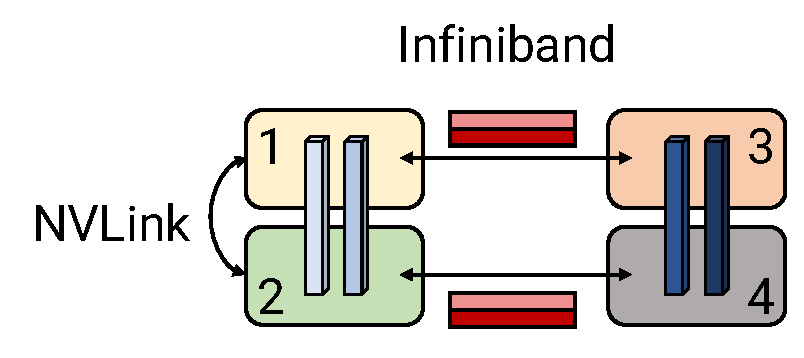
\includegraphics[keepaspectratio=1.0,width=\columnwidth]{figures/without_scatter_gather_optimization.pdf}
        \caption{W/o scatter/gather optimization.}
        \label{fig:without_scatter_gather_optimization}
    \end{subfigure}
    \begin{subfigure}[c]{0.49\columnwidth}
        \centering
        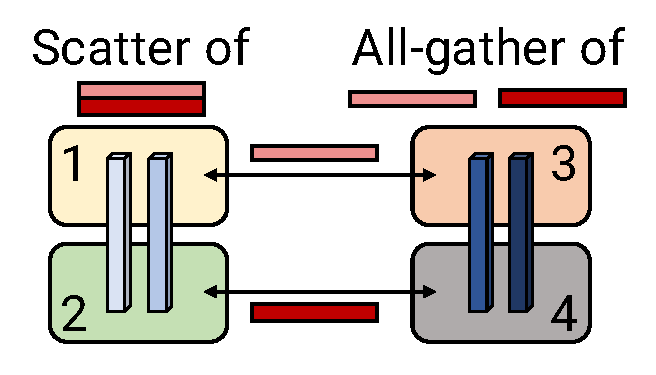
\includegraphics[keepaspectratio=1.0,width=0.78\columnwidth]{figures/with_scatter_gather_optimization.pdf}
        \caption{With scatter/gather optimization.}
        \label{fig:with_scatter_gather_optimization}
    \end{subfigure}
    \vspace{-0.1in}
    \caption{
        Scatter/gather communication optimization. Light blue blocks are layers in the first pipeline stage, and dark blue blocks are layers in the second pipeline stage. Without the scatter/gather optimization, the same tensor is sent redundantly over inter-node InfiniBand links. Instead, at the sender, we can scatter the tensor into smaller chunks, reducing the sizes of tensors sent over InfiniBand links. The final tensor can then be rematerialized at the receiver using a gather operation.
    }
    \label{fig:scatter_gather_optimization}
\end{figure}

\subsection{Communication Optimizations}

When using pipeline parallelism, we want to send and receive tensors in the forward and backward direction in parallel. Each DGX A100 is equipped with 8 InfiniBand (IB) networking cards. Unfortunately, sends and receives are point-to-point, and only happen between a pair of GPUs on two servers, making it hard to leverage all 8 cards for a single communication call within the pipeline.

However, we can leverage the fact that we use both tensor model parallelism and pipeline model parallelism to reduce the overhead of cross-node communication. In particular, we note that the output of each transformer layer is replicated (after $g$ in MLP block, see Figure \ref{fig:tensor_model_parallelism_mlp}) across the tensor-parallel ranks. As a result, ranks in two consecutive pipeline stages that are performing tensor model parallelism send and receive the exact same set of tensors (Figure~\ref{fig:without_scatter_gather_optimization}).

For large enough models, we use a tensor-model-parallel size of 8. This means we are sending the same set of tensors 8 times between corresponding GPUs on adjacent multi-GPU servers. To reduce this redundancy, we can instead split the tensor on the send side into equal-sized chunks, and then only send one chunk to the corresponding rank on the next node using the rank's own InfiniBand card (e.g., rank 1 sends to rank 3 and rank 2 sends to rank 4 in Figure~\ref{fig:scatter_gather_optimization}). With 8 tensor-model-parallel ranks, each chunk would be one-eighth smaller. Then, on the receive side, we can perform an all-gather over NVLink, which is much faster than the InfiniBand interconnect, to re-materialize the full tensor. This is shown in Figure~\ref{fig:with_scatter_gather_optimization}. We call this the \emph{scatter/gather communication optimization}. This optimization helps better leverage the multiple IB cards on the DGX A100 servers, and makes more communication-intensive schedules such as the interleaved one feasible.

Quantitatively, with the scatter-gather communication optimization, the total amount of communication that needs to be performed between every pair of consecutive stages is reduced to $\frac{bsh}{t}$, where $t$ is the tensor-model-parallel size, $s$ is the sequence length, and $h$ is the hidden size ($t=8$ in our experiments).

\subsection{Computation Optimizations}
\label{sec:computation_optimizations}

We implemented three model-specific optimizations to the computation graph to attain high performance. First, we changed the data layout in the transformer layer to avoid memory-intensive transpose operations, and to enable the use of strided batched GEMM kernels. Specifically, we changed the data layout from $[b, s, a, h]$ to $[s, b, a, h]$, where $b$, $s$, $a$, and $h$ are batch, sequence, attention-head, and hidden-size dimensions, respectively. Second, we generated fused kernels for a sequence of element-wise operations (bias + GeLU and bias + dropout + add) using PyTorch JIT~\cite{pytorchjit}. Third, we created two custom kernels to enable the fusion of scale, mask, and softmax (reduction) operations: one to support general masking (used in models such as BERT) and another to support implicit causal masking (used in auto-regressive models such as GPT). We quantify the effect of these optimizations in the next section.
